\hypertarget{appendix-appendix}{%
\appendix}


\hypertarget{anatomical-terms-of-location}{%
\chapter{Anatomical Terms Of Location}\label{anatomical-terms-of-location}}

All vertebrates (including humans) have the same basic body plan -- they are strictly bilaterally symmetrical in early embryonic stages and largely bilaterally symmetrical in adulthood. That is, they have mirror-image left and right halves if divided down the middle. For these reasons, the basic directional terms can be considered to be those used in vertebrates. By extension, the same terms are used for many other (invertebrate) organisms as well.

Standardized anatomical and zoological terms of location have been developed, usually based on Latin and Greek words, to enable all biological and medical scientists to precisely delineate and communicate information about animal bodies and their component organs, even though the meaning of some of the terms often is context-sensitive.

The vertebrates and Craniata share a substantial heritage and common structure, so many of the same terms are used for location. To avoid ambiguities this terminology is based on the anatomy of each animal in a standard way.

While these terms are standardized within specific fields of biology, there are unavoidable, sometimes dramatic differences between some disciplines. For example, differences in terminology remain a problem that, to some extent, still separates the terminology of human anatomy from that used in the study of various other zoological categories.

For humans, one type of vertebrate, anatomical terms may differ from other forms of vertebrates. For one reason, this is because humans have a different neuraxis and, unlike animals that rest on four limbs, humans are considered when describing anatomy as being in the standard anatomical position. Thus what is on ``top'' of a human is the head, whereas the ``top'' of a dog may be its back, and the ``top'' of a flounder could refer to either its left or its right side.

\hypertarget{anatomical-planes}{%
\section{Anatomical Planes}\label{anatomical-planes}}

Anatomical planes

\begin{itemize}
\tightlist
\item
  A transverse plane, also known as a cross-section, divides the body into cranial and caudal (head and tail) portions.
\item
  A longitudinal plane is any plane that is perpendicular to the transverse plane. The main longitudinal planes are:

  \begin{itemize}
  \tightlist
  \item
    The frontal plane or coronal plane divides the body into dorsal and ventral (back and front, or posterior and anterior) portions. For post-embryonic humans a coronal plane is vertical and a transverse plane is horizontal, but for embryos and quadrupeds a coronal plane is horizontal and a transverse plane is vertical.
  \item
    The sagittal plane is a plane parallel to the sagittal suture. All other sagittal planes (referred to as parasagittal planes) are parallel to it. The plane is a Y-Z plane, perpendicular to the ground. A special sagittal plane is the median plane or midsagittal plane in the midline of the body, and divides the body into left and right (sinister and dexter) portions. This passes through the head, spinal cord, navel, and, in many animals, the tail. The term ``median plane'' can also refer to the midsagittal plane of other structures, such as a digit.
  \end{itemize}
\end{itemize}

\hypertarget{anatomical-axes}{%
\section{Anatomical Axes}\label{anatomical-axes}}

To begin with, distinct, polar-opposite ends of the organism are chosen. By definition, each pair of opposite points defines an axis. In a bilaterally symmetrical organism, there are 6 polar opposite points, giving three axes that intersect at right angles -- the x, y, and z axes familiar from three-dimensional geometry.
\onecolumn
\begin{longtable}[t]{>{\raggedright\arraybackslash}p{15em}>{\raggedright\arraybackslash}p{10em}>{\raggedright\arraybackslash}p{10em}}
\caption{\label{tab:axes}The main anatomical axes.}\\
\toprule
Axis & Directional term & Directed towards\\
\midrule
\rowcolor{gray!6}   &  & Belly in orthograde bipeds (including humans)\\

\multirow{-2}{15em}{\raggedright\arraybackslash Anteroposterior} & \multirow{-2}{10em}{\raggedright\arraybackslash Anterior} & Head end in fish\\
\cmidrule{1-3}
\rowcolor{gray!6}   & Back in orthograde bipeds & \\

\multirow{-2}{15em}{\raggedright\arraybackslash Posterior} & Rear/tail end & \\
\cmidrule{1-3}
\rowcolor{gray!6}  Rostrocaudal, craniocaudal, cephalocaudal,  longitudinal & Rostral, cranial, cephalad & Head end\\
\cmidrule{1-3}
 & Rear/tail end & \\

\rowcolor{gray!6}  \multirow{-2}{15em}{\raggedright\arraybackslash Caudal} & Inferior in humans & \\
\cmidrule{1-3}
Dorsoventral & Dorsal & Back, spinal column\\
\cmidrule{1-3}
\rowcolor{gray!6}  Ventral & Belly & \\
\cmidrule{1-3}
Left-right, dextro-sinister, sinistro-dexter & Left (sinister) & Left-hand side\\
\cmidrule{1-3}
\rowcolor{gray!6}  Right (dexter) & Right-hand side & \\
\cmidrule{1-3}
Mediolateral & Medial & Centre\\
\cmidrule{1-3}
\rowcolor{gray!6}  Lateral & Left and right & \\
\cmidrule{1-3}
Proximal/distal & Proximal & Point at which appendage joins the body\\
\cmidrule{1-3}
\rowcolor{gray!6}  Distal & Extremity of appendage & \\
\bottomrule
\end{longtable}
\twocolumn
The terms ``intermediate'', ``ipsilateral'', ``contralateral'', ``superficial'', and ``deep'', while indicating directions, are relative terms and thus do not properly define fixed anatomical axes. Also, while the ``rostrocaudal'' and anteroposterior directionality are equivalent in a significant portion of the human body, they are different directions in other parts of the body.

\hypertarget{main-anatomical-terms}{%
\section{Main Anatomical Terms}\label{main-anatomical-terms}}

\hypertarget{superior-and-inferior}{%
\subsection{Superior And Inferior}\label{superior-and-inferior}}

In anatomical terminology superior (from Latin, meaning `above') is used to refer to what is above something, and inferior (from Latin, meaning `below') to what is below it. For example, in the anatomical position the most superior part of the human body is the head, and the most inferior is the feet. As a second example, in humans the neck is superior to the chest but inferior to the head.

\hypertarget{anterior-and-posterior}{%
\subsection{Anterior And Posterior}\label{anterior-and-posterior}}

Anterior refers to what is in front (from Latin ante, meaning ``before'') and posterior, what is to the back of the subject (from Latin post, meaning ``after''). For example, in a dog the nose is anterior to the eyes and the tail is considered the most posterior part; in many fish the gill openings are posterior to the eyes, but anterior to the tail. In projectional radiography terminology, an anteroposterior (AP) projection is taken with the X-ray generator anteriorly (such as in the front of a human), and the X-ray detector posteriorly. In contrast, a posteroanterior (PA) projection is taken with the X-ray generator posteriorly.

\hypertarget{medial-and-lateral}{%
\subsection{Medial And Lateral}\label{medial-and-lateral}}

Lateral (from Latin lateralis, meaning `to the side') refers to the sides of an animal, as in ``left lateral'' and ``right lateral''. The term medial (from Latin medius, meaning `middle') is used to refer to structures close to the centre of an organism, called the ``median plane''. For example, in a human, imagine a line down the center of the body from the head though the navel and going between the legs--- the medial side of the foot would be the big toe side; the medial side of the knee would be the side adjacent to the other knee. To describe the sides of the knees touching each other would be ``right medial'' and ``left medial''.

The terms ``left'' and ``right'' are sometimes used, or their Latin alternatives (Latin: dexter; ``right'', Latin: sinister; ``left''). However, as left and right sides are mirror images, using these words is somewhat confusing, as structures are duplicated on both sides. For example, it is very confusing to say the dorsal fin of a dolphin is ``right of'' the left pectoral fin, but is ``left of'' the right eye, but much easier and clearer to say ``the dorsal fin is medial to the pectoral fins''.

Terms derived from lateral include:

\begin{itemize}
\tightlist
\item
  Contralateral (from Latin contra, meaning `against'): on the side opposite to another structure. For example, the right arm and leg are represented by the left, i.e., contralateral side of the forebrain.
\item
  Ipsilateral (from Latin ipse, meaning `same'): on the same side as another structure. For example, the left arm is ipsilateral to the left leg.
\item
  Bilateral (from Latin bis, meaning `twice'): on both sides of the body. For example, bilateral orchiectomy (removal of testes on both sides of the body's axis) is surgical castration.
\item
  Unilateral (from Latin unus, meaning `one'): on one side of the body. For example, unilateral paresis is hemiparesis.
\end{itemize}

Terms derived from medial include:

\begin{itemize}
\item
  Inferomedial (from Latin inferus, meaning `lower'): lower and in or near the midline. For example, the human nose is inferomedial to the eyes.
\item
\begin{verbatim}
  Superomedial (from Latin superus, meaning 'above'): above and toward the midline. For example, the human nose is superomedial to the mouth.
\end{verbatim}
\end{itemize}

\hypertarget{central-and-peripheral}{%
\subsection{Central And Peripheral}\label{central-and-peripheral}}

Central and peripheral are terms that are closely related to concepts such as proximal and distal, but they are so widely applicable that in many respects their flexibility makes them hard to define. Loosely speaking, they distinguish near and far, inside and out, or even organs of vital importance such as heart and lungs, from peripheral organs such as fingers, that undoubtedly may be important, but which it may not be life-threatening to dispense with. Examples of the application of the terms are the distinction between central- and peripheral nervous systems, and between peripheral blood vessels and the central circulatory organs, such as the heart and major vessels. The terms also can apply to large and complex molecules such as proteins, where central amino acid residues are protected from antibodies or the like, but peripheral residues are important in docking and other interactions. Other examples include Central and peripheral circadian clocks, and central versus peripheral vision.

\hypertarget{superficial-and-deep}{%
\subsection{Superficial And Deep}\label{superficial-and-deep}}

These two terms relate to the distance of a structure from the surface of an animal.

Deep (from Old English) refers to something further away from the surface of the organism. For example, the external oblique muscle of the abdomen is deep to the skin. ``Deep'' is one of the few anatomical terms of location derived from Old English rather than Latin -- the anglicised Latin term would have been ``profound'' (from Latin profundus, meaning `due to depth').

Superficial (from Latin superficies, meaning `surface') refers to something near the outer surface of the organism. For example, in skin the epidermis is superficial to the subcutis.

\hypertarget{dorsal-and-ventral}{%
\subsection{Dorsal And Ventral}\label{dorsal-and-ventral}}

These two terms, used in anatomy and embryology, refer to back (dorsal) and front or belly (ventral) of an organism.

The dorsal (from Latin dorsum, meaning `back') surface of an organism refers to the back, or upper side, of an organism. If talking about the skull, the dorsal side is the top.

The ventral (from Latin venter, meaning `belly') surface refers to the front, or lower side, of an organism.

For example, in a fish the pectoral fins are dorsal to the anal fin, but ventral to the dorsal fin.

\hypertarget{cranial-and-caudal}{%
\subsubsection{Cranial And Caudal}\label{cranial-and-caudal}}



\begin{figure}

{\centering 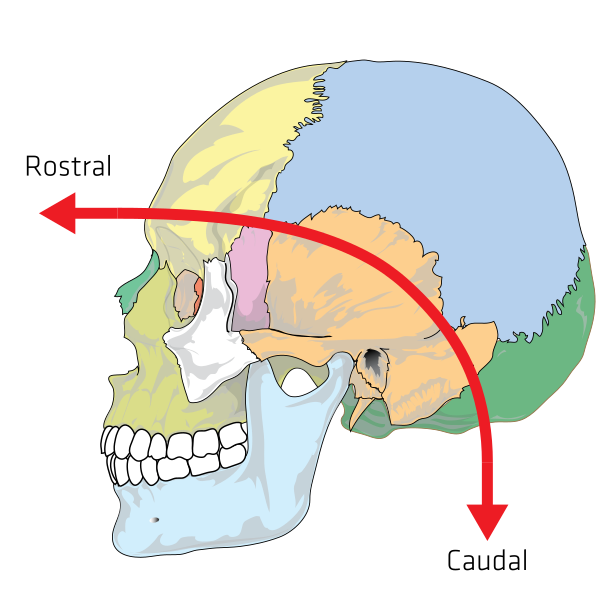
\includegraphics[width=0.7\linewidth]{./figures/appendix/Rostralcaudal} 

}

\caption{\href{https://commons.wikimedia.org/wiki/File:Rostralcaudal.svg}{In the human skull the terms rostral and caudal are adapted to the curved neuraxis of Hominidae}}\label{fig:rostralcaudal}
\end{figure}

Specific terms exist to describe how close or far something is to the head or tail of an animal. To describe how close to the head of an animal something is, three distinct terms are used:

\begin{itemize}
\tightlist
\item
  Rostral (from Latin rostrum, meaning `beak, nose'), meaning situated toward the oral or nasal region, or in the case of the brain, toward the tip of the frontal lobe.
\item
  Cranial (from Greek κρανίον, meaning `skull') or cephalic (from Greek κεφαλή, meaning `head').
\item
  Caudal (from Latin cauda, meaning `tail') is used to describe how close something is to the trailing end of an organism,
  For example, in the horse, the eyes are caudal to the nose and rostral to the back of the head.
\end{itemize}

These terms are generally preferred in veterinary medicine and not used as often in human medicine. In humans, ``cranial'' and ``cephalic'' are used to refer to the skull, with ``cranial'' being used more commonly. The term ``rostral'' is rarely used in human anatomy, apart from embryology, and refers more to the front of the face than the superior aspect of the organism. Similarly, the term ``caudal'' is only occasionally used in human anatomy. This is because the brain is situated at the superior part of the head whereas the nose is situated in the anterior part. Thus the ``rostrocaudal axis'' refers to a C shape (see image).

The location of anatomical structures can also be described with relation to different anatomical landmarks.

Structures may be described as being at the level of a specific spinal vertebra, depending on the section of the vertebral column the structure is at. The position is often abbreviated. For example, structures at the level of the fourth cervical vertebra may be abbreviated as ``C4'', at the level of the fourth thoracic vertebra ``T4'', and at the level of the third lumbar vertebra ``L3''. Because the sacrum and coccyx are fused, they are not often used to provide location.

Directional and locational prefixes can modify many anatomical and morphological terms, sometimes in formally standard usage, but often attached arbitrarily according to need or convenience.

Several other terms are also used to describe location. These terms are not used to form the fixed axes. Terms include:

\begin{itemize}
\tightlist
\item
  Axial (from Latin axis, meaning `axle'): around the central axis of the organism or the extremity. Two related terms, ``abaxial'' and ``adaxial'', refer to locations away from and toward the central axis of an organism, respectively
\item
  Parietal (from Latin paries, meaning `wall'): pertaining to the wall of a body cavity. For example, the parietal peritoneum is the lining on the inside of the abdominal cavity. Parietal can also refer specifically to the parietal bone of the skull or associated structures.
\item
  Posteromedial (from Latin posterus, meaning `coming after', and medius, meaning `middle'): situated towards the middle of the posterior surface.
\item
  Posterosuperior (from Latin posterus, meaning `coming after' and superior): situated towards the upper part of the posterior surface.
\item
  Terminal (from Latin terminus, meaning `boundary or end') at the extremity of a (usually projecting) structure, as in ``\ldots an antenna with a terminal sensory hair''.
\item
  Visceral and viscus (from Latin viscera, meaning `internal organs'): associated with organs within the body's cavities. For example, the stomach is covered with a lining called the visceral peritoneum as opposed to the parietal peritoneum. Viscus can also be used to mean ``organ''. For example, the stomach is a viscus within the abdominal cavity.
\end{itemize}

\hypertarget{prefixes}{%
\section{Prefixes}\label{prefixes}}

\begin{itemize}
\tightlist
\item
  Sub- (from Latin sub, meaning `preposition beneath, close to, nearly etc') appended as a prefix, with or without the hyphen, qualifies terms in various senses. Consider subcutaneous as meaning beneath the skin, subterminal meaning near to the end of a structure. Sub- also may mean ``nearly'' or ``more-or-less''; for instance subglobular means almost globular. In many usages sub- is similar in application to ``hypo-''
\item
  Hypo- (from Ancient Greek ὑπό, meaning `under') Like ``sub'' in various senses as in hypolingual nerve beneath the tongue, or hypodermal fat beneath the skin
\item
  Infra- (from Latin infra, meaning `preposition beneath, below etc') Similar to ``sub''; a direct opposite to super- and supra-, as in Infratemporal space or infraorbital.
\item
  Inter- (from Latin inter, meaning `between'): between two other structures. For example, the navel is intermediate to the left arm and the contralateral (right) leg. The intercostal muscles run between the ribs.
\item
  Super- or Supra- (from Latin super, supra, meaning `above, on top of, beyond etc') appended as a prefix, with or without the hyphen, as in superciliary arches or supraorbital
\end{itemize}

\hypertarget{neuroanatomical-terms}{%
\chapter{Neuroanatomical Terms}\label{neuroanatomical-terms}}

\hypertarget{nucleus}{%
\section{Nucleus}\label{nucleus}}

In neuroanatomy, a nucleus (plural form: nuclei) is a cluster of neurons in the central nervous system, located deep within the cerebral hemispheres and brainstem. The neurons in one nucleus usually have roughly similar connections and functions. Nuclei are connected to other nuclei by tracts, the bundles (fascicles) of axons (nerve fibers) extending from the cell bodies. A nucleus is one of the two most common forms of nerve cell organization, the other being layered structures such as the cerebral cortex or cerebellar cortex. In anatomical sections, a nucleus shows up as a region of gray matter, often bordered by white matter. The vertebrate brain contains hundreds of distinguishable nuclei, varying widely in shape and size. A nucleus may itself have a complex internal structure, with multiple types of neurons arranged in clumps (subnuclei) or layers.

The term ``nucleus'' is in some cases used rather loosely, to mean simply an identifiably distinct group of neurons, even if they are spread over an extended area. The reticular nucleus of the thalamus, for example, is a thin layer of inhibitory neurons that surrounds the thalamus.

Some of the major anatomical components of the brain are organized as clusters of interconnected nuclei. Notable among these are the thalamus and hypothalamus, each of which contains several dozen distinguishable substructures. The medulla and pons also contain numerous small nuclei with a wide variety of sensory, motor, and regulatory functions.

In the peripheral nervous system (PNS), a cluster of cell bodies of neurons (homologous to a CNS nucleus) is called a ganglion. The fascicles of nerve fibers in the PNS (homologous to CNS tracts) are called nerves.

\hypertarget{ganglion}{%
\section{Ganglion}\label{ganglion}}

A ganglion is a group of neuron cell bodies in the peripheral nervous system. In the somatic nervous system this includes dorsal root ganglia and trigeminal ganglia among a few others. In the autonomic nervous system there are both sympathetic and parasympathetic ganglia which contain the cell bodies of postganglionic sympathetic and parasympathetic neurons respectively.

Ganglia are primarily made up of somata and dendritic structures which are bundled or connected. Ganglia often interconnect with other ganglia to form a complex system of ganglia known as a plexus. Ganglia provide relay points and intermediary connections between different neurological structures in the body, such as the peripheral and central nervous systems.

Among vertebrates there are three major groups of ganglia:

\begin{itemize}
\tightlist
\item
  Dorsal root ganglia (also known as the spinal ganglia) contain the cell bodies of sensory (afferent) neurons.
\item
  Cranial nerve ganglia contain the cell bodies of cranial nerve neurons.
\item
  Autonomic ganglia contain the cell bodies of autonomic nerves.
\end{itemize}

In the autonomic nervous system, fibers from the central nervous system to the ganglia are known as preganglionic fibers, while those from the ganglia to the effector organ are called postganglionic fibers.

Basal ganglia
The term ``ganglion'' refers to the peripheral nervous system.

However, in the brain (part of the central nervous system), the ``basal ganglia'' is a group of nuclei interconnected with the cerebral cortex, thalamus, and brainstem, associated with a variety of functions: motor control, cognition, emotions, and learning.

Partly due to this ambiguity, the Terminologia Anatomica recommends using the term basal nuclei instead of basal ganglia; however, this usage has not been generally adopted.

\hypertarget{tract}{%
\section{Tract}\label{tract}}

A nerve tract is a bundle of nerve fibers (axons) connecting nuclei of the central nervous system. In the peripheral nervous system this is known as a nerve, and has associated connective tissue. The main nerve tracts in the central nervous system are of three types: association fibers, commissural fibers, and projection fibers. A tract may also be referred to as a commissure, fasciculus or decussation. A commissure connects the two cerebral hemispheres at the same levels. Examples are the posterior commissure and the corpus callosum. A decussation is a connection made by fibres that cross at different levels (obliquely), such as the sensory decussation. Examples of a fascicle are the subthalamic fasciculus and the lenticular fasciculus.

In the brain, bundles of axons are also categorized by their function into association fibers, projection fibers, and commissural fibers.

\hypertarget{lemniscus}{%
\section{Lemniscus}\label{lemniscus}}

A lemniscus (Greek for ribbon or band) is a bundle of secondary sensory fibres in the brainstem. The medial lemniscus and lateral lemniscus terminate in specific relay nuclei of the diencephalon. The trigeminal lemniscus is sometimes considered as the cephalic part of the medial lemniscus.

\hypertarget{list-of-regions-in-the-human-brain}{%
\chapter{List Of Regions In The Human Brain}\label{list-of-regions-in-the-human-brain}}

\hypertarget{hindbrain-rhombencephalon}{%
\section{Hindbrain (rhombencephalon)}\label{hindbrain-rhombencephalon}}

Myelencephalon

\begin{itemize}
\tightlist
\item
  Medulla oblongata
\item
  Medullary pyramids
\item
  Olivary body
\item
  Inferior olivary nucleus
\item
  Rostral ventrolateral medulla
\item
  Caudal ventrolateral medulla
\item
  Solitary nucleus (Nucleus of the solitary tract)
\item
  Respiratory center-Respiratory groups

  \begin{itemize}
  \tightlist
  \item
    Dorsal respiratory group
  \item
    Ventral respiratory group or Apneustic centre

    \begin{itemize}
    \tightlist
    \item
      Pre-Bötzinger complex
    \item
      Bötzinger complex
    \item
      Retrotrapezoid nucleus
    \item
      Nucleus retrofacialis
    \item
      Nucleus retroambiguus
    \item
      Nucleus para-ambiguus
    \end{itemize}
  \end{itemize}
\item
  Paramedian reticular nucleus
\item
  Gigantocellular reticular nucleus
\item
  Parafacial zone
\item
  Cuneate nucleus
\item
  Gracile nucleus
\item
  Perihypoglossal nuclei

  \begin{itemize}
  \tightlist
  \item
    Intercalated nucleus
  \item
    Prepositus nucleus
  \item
    Sublingual nucleus
  \end{itemize}
\item
  Area postrema
\item
  Medullary cranial nerve nuclei

  \begin{itemize}
  \tightlist
  \item
    Inferior salivatory nucleus
  \item
    Nucleus ambiguus
  \item
    Dorsal nucleus of vagus nerve
  \item
    Hypoglossal nucleus
  \end{itemize}
\item
  Chemoreceptor trigger zone
\end{itemize}

Metencephalon

\begin{itemize}
\tightlist
\item
  Pons

  \begin{itemize}
  \tightlist
  \item
    Pontine nuclei
  \item
    Pontine cranial nerve nuclei
  \item
    chief or pontine nucleus of the trigeminal nerve sensory nucleus (V)
  \item
    Motor nucleus for the trigeminal nerve (V)
  \item
    Abducens nucleus (VI)
  \item
    Facial nerve nucleus (VII)
  \item
    vestibulocochlear nuclei (vestibular nuclei and cochlear nuclei) (VIII)
  \item
    Superior salivatory nucleus
  \end{itemize}
\item
  Pontine tegmentum

  \begin{itemize}
  \tightlist
  \item
    Pontine micturition center (Barrington's nucleus)
  \item
    Locus coeruleus
  \item
    Pedunculopontine nucleus
  \item
    Laterodorsal tegmental nucleus
  \item
    Tegmental pontine reticular nucleus
  \item
    Nucleus incertus
  \end{itemize}
\item
  Parabrachial area

  \begin{itemize}
  \tightlist
  \item
    Medial parabrachial nucleus
  \item
    Lateral parabrachial nucleus
  \item
    Subparabrachial nucleus (Kölliker-Fuse nucleus)

    \begin{itemize}
    \tightlist
    \item
      Pontine respiratory group
    \end{itemize}
  \end{itemize}
\item
  Superior olivary complex

  \begin{itemize}
  \tightlist
  \item
    Medial superior olive
  \item
    Lateral superior olive
  \item
    Medial nucleus of the trapezoid body
  \end{itemize}
\item
  Paramedian pontine reticular formation
\item
  Parvocellular reticular nucleus
\item
  Caudal pontine reticular nucleus
\item
  Cerebellar peduncles

  \begin{itemize}
  \tightlist
  \item
    Superior cerebellar peduncle
  \item
    Middle cerebellar peduncle
  \item
    Inferior cerebellar peduncle
  \item
    Fourth ventricle
  \end{itemize}
\item
  Cerebellum

  \begin{itemize}
  \tightlist
  \item
    Cerebellar vermis
  \item
    Cerebellar hemispheres

    \begin{itemize}
    \tightlist
    \item
      Anterior lobe
    \item
      Posterior lobe
    \item
      Flocculonodular lobe
    \end{itemize}
  \end{itemize}
\item
  Cerebellar nuclei

  \begin{itemize}
  \tightlist
  \item
    Fastigial nucleus
  \item
    Interposed nucleus

    \begin{itemize}
    \tightlist
    \item
      Globose nucleus
    \item
      Emboliform nucleus
    \end{itemize}
  \item
    Dentate nucleus
  \end{itemize}
\end{itemize}

\hypertarget{midbrain-mesencephalon}{%
\section{Midbrain (mesencephalon)}\label{midbrain-mesencephalon}}

\begin{itemize}
\tightlist
\item
  Tectum

  \begin{itemize}
  \tightlist
  \item
    Corpora quadrigemina

    \begin{itemize}
    \tightlist
    \item
      inferior colliculi
    \item
      superior colliculi
    \end{itemize}
  \end{itemize}
\item
  Pretectum
\item
  Tegmentum

  \begin{itemize}
  \tightlist
  \item
    Periaqueductal gray
  \item
    Rostral interstitial nucleus of medial longitudinal fasciculus
  \item
    Midbrain reticular formation
  \item
    Dorsal raphe nucleus
  \item
    Red nucleus
  \item
    Ventral tegmental area

    \begin{itemize}
    \tightlist
    \item
      Parabrachial pigmented nucleus
    \item
      Paranigral nucleus
    \item
      Rostromedial tegmental nucleus
    \end{itemize}
  \item
    Caudal linear nucleus
  \item
    Rostral linear nucleus of the raphe
  \item
    Interfascicular nucleus
  \item
    Substantia nigra

    \begin{itemize}
    \tightlist
    \item
      Pars compacta
    \item
      Pars reticulata
    \end{itemize}
  \item
    Interpeduncular nucleus
  \end{itemize}
\item
  Cerebral peduncle

  \begin{itemize}
  \tightlist
  \item
    Crus cerebri
  \end{itemize}
\item
  Mesencephalic cranial nerve nuclei

  \begin{itemize}
  \tightlist
  \item
    Oculomotor nucleus (III)
  \item
    Edinger-Westphal nucleus
  \item
    Trochlear nucleus (IV)
  \end{itemize}
\item
  Mesencephalic duct (cerebral aqueduct, aqueduct of Sylvius)
\end{itemize}

\hypertarget{forebrain-prosencephalon}{%
\section{Forebrain (prosencephalon)}\label{forebrain-prosencephalon}}

Diencephalon

Epithalamus

\begin{itemize}
\tightlist
\item
  Pineal body (pineal gland)
\item
  Habenular nuclei
\item
  Stria medullaris
\item
  Taenia thalami
\end{itemize}

Third ventricle

\begin{itemize}
\tightlist
\item
  Subcommissural organ
\end{itemize}

Thalamus

\begin{itemize}
\tightlist
\item
  Anterior nuclear group

  \begin{itemize}
  \tightlist
  \item
    Anteroventral nucleus (a.k.a. ventral anterior nucleus)
  \item
    Anterodorsal nucleus
  \item
    Anteromedial nucleus
  \end{itemize}
\item
  Medial nuclear group

  \begin{itemize}
  \tightlist
  \item
    Medial dorsal nucleus
  \item
    Midline nuclear group
  \item
    Paratenial nucleus
  \item
    Reuniens nucleus
  \item
    Rhomboidal nucleus
  \item
    Intralaminar nuclear group
  \item
    Centromedian nucleus
  \item
    Parafascicular nucleus
  \item
    Paracentral nucleus
  \item
    Central lateral nucleus
  \end{itemize}
\item
  Lateral nuclear group

  \begin{itemize}
  \tightlist
  \item
    Lateral dorsal nucleus
  \item
    Lateral posterior nucleus
  \item
    Pulvinar

    \begin{itemize}
    \tightlist
    \item
      anterior pulvinar nucleus
    \item
      lateral pulvinar nucleus
    \item
      medial pulvinar nucleus
    \item
      inferior pulvinar nucleus
    \end{itemize}
  \end{itemize}
\item
  Ventral nuclear group

  \begin{itemize}
  \tightlist
  \item
    Ventral anterior nucleus
  \item
    Ventral lateral nucleus
  \item
    Ventral posterior nucleus

    \begin{itemize}
    \tightlist
    \item
      Ventral posterior lateral nucleus
    \item
      Ventral posterior medial nucleus
    \end{itemize}
  \item
    Medial geniculate body
  \item
    Lateral geniculate body
  \end{itemize}
\item
  Thalamic reticular nucleus
\end{itemize}

Hypothalamus (limbic system) (HPA axis)

\begin{itemize}
\tightlist
\item
  Anterior

  \begin{itemize}
  \tightlist
  \item
    Medial area

    \begin{itemize}
    \tightlist
    \item
      Parts of preoptic area

      \begin{itemize}
      \tightlist
      \item
        Medial preoptic nucleus

        \begin{itemize}
        \tightlist
        \item
          INAH 1
        \item
          INAH 2
        \item
          INAH 3
        \item
          INAH 4
        \end{itemize}
      \end{itemize}
    \item
      Suprachiasmatic nucleus
    \item
      Paraventricular nucleus
    \item
      Supraoptic nucleus (mainly)
    \item
      Anterior hypothalamic nucleus
    \end{itemize}
  \item
    Lateral area
  \item
    Parts of preoptic area
  \item
    Lateral preoptic nucleus
  \item
    Anterior part of Lateral nucleus
  \item
    Part of supraoptic nucleus
  \item
    Other nuclei of preoptic area

    \begin{itemize}
    \tightlist
    \item
      median preoptic nucleus
    \item
      periventricular preoptic nucleus
    \end{itemize}
  \end{itemize}
\item
  Tuberal

  \begin{itemize}
  \tightlist
  \item
    Medial area

    \begin{itemize}
    \tightlist
    \item
      Dorsomedial hypothalamic nucleus
    \item
      Ventromedial nucleus
    \item
      Arcuate nucleus
    \end{itemize}
  \item
    Lateral area

    \begin{itemize}
    \tightlist
    \item
      Tuberal part of Lateral nucleus
    \item
      Lateral tuberal nuclei
    \end{itemize}
  \end{itemize}
\item
  Posterior

  \begin{itemize}
  \tightlist
  \item
    Medial area

    \begin{itemize}
    \tightlist
    \item
      Mammillary nuclei (part of mammillary bodies)
    \item
      Posterior nucleus
    \end{itemize}
  \item
    Lateral area

    \begin{itemize}
    \tightlist
    \item
      Posterior part of Lateral nucleus
    \end{itemize}
  \end{itemize}
\item
  Surface

  \begin{itemize}
  \tightlist
  \item
    Median eminence
  \item
    Mammillary bodies
  \item
    Pituitary stalk (infundibulum)
  \end{itemize}
\item
  Optic chiasm
\item
  Subfornical organ
\item
  Periventricular nucleus
\item
  Tuber cinereum

  \begin{itemize}
  \tightlist
  \item
    Tuberal nucleus
  \item
    Tuberomammillary nucleus
  \end{itemize}
\item
  Tuberal region
\item
  Mammillary nucleus
\end{itemize}

Subthalamus(HPA axis)

\begin{itemize}
\tightlist
\item
  Subthalamic nucleus
\item
  Zona incerta
\end{itemize}

Pituitary gland (HPA axis)

\begin{itemize}
\tightlist
\item
  neurohypophysis
\item
  Pars intermedia (Intermediate Lobe)
\item
  adenohypophysis
\end{itemize}

Telencephalon (cerebrum) Cerebral hemispheres

White matter

\begin{itemize}
\tightlist
\item
  Centrum semiovale
\item
  Corona radiata
\item
  Internal capsule
\item
  External capsule
\item
  Extreme capsule
\end{itemize}

Subcortical

\begin{itemize}
\tightlist
\item
  Hippocampus (Medial Temporal Lobe)

  \begin{itemize}
  \tightlist
  \item
    Dentate gyrus
  \item
    Cornu ammonis (CA fields)

    \begin{itemize}
    \tightlist
    \item
      Cornu ammonis area 1 (CA1)
    \item
      Cornu ammonis area 2 (CA2)
    \item
      Cornu ammonis area 3 (CA3)
    \item
      Cornu ammonis area 4 (CA4)
    \end{itemize}
  \end{itemize}
\item
  Amygdala (limbic system) (limbic lobe)

  \begin{itemize}
  \tightlist
  \item
    Central nucleus (autonomic nervous system)
  \item
    Medial nucleus (accessory olfactory system)
  \item
    Cortical and basomedial nuclei (main olfactory system)
  \item
    Lateral and basolateral nuclei (frontotemporal cortical system)
  \end{itemize}
\item
  Extended amygdala

  \begin{itemize}
  \tightlist
  \item
    Stria terminalis

    \begin{itemize}
    \tightlist
    \item
      Bed nucleus of the stria terminalis
    \end{itemize}
  \end{itemize}
\item
  Claustrum
\item
  Basal ganglia

  \begin{itemize}
  \tightlist
  \item
    Striatum

    \begin{itemize}
    \tightlist
    \item
      Dorsal striatum (a.k.a. neostriatum)

      \begin{itemize}
      \tightlist
      \item
        Putamen
      \item
        Caudate nucleus
      \end{itemize}
    \item
      Ventral striatum

      \begin{itemize}
      \tightlist
      \item
        Nucleus accumbens
      \item
        Olfactory tubercle
      \end{itemize}
    \item
      Globus pallidus (forms nucleus lentiformis with putamen)

      \begin{itemize}
      \tightlist
      \item
        Ventral pallidum
      \end{itemize}
    \item
      Subthalamic nucleus
    \end{itemize}
  \end{itemize}
\item
  Basal forebrain

  \begin{itemize}
  \tightlist
  \item
    Anterior perforated substance
  \item
    Substantia innominata
  \item
    Nucleus basalis
  \item
    Diagonal band of Broca
  \item
    Septal nuclei

    \begin{itemize}
    \tightlist
    \item
      Medial septal nuclei
    \end{itemize}
  \item
    Lamina terminalis

    \begin{itemize}
    \tightlist
    \item
      Vascular organ of lamina terminalis
    \end{itemize}
  \end{itemize}
\end{itemize}

Rhinencephalon (paleocortex)

\begin{itemize}
\tightlist
\item
  Olfactory bulb
\item
  Olfactory tract
\item
  Anterior olfactory nucleus
\item
  Piriform cortex
\item
  Anterior commissure
\item
  Uncus
\item
  Periamygdaloid cortex
\end{itemize}

Cerebral cortex (neocortex)

\begin{itemize}
\tightlist
\item
  Frontal lobe

  \begin{itemize}
  \tightlist
  \item
    Cortex

    \begin{itemize}
    \tightlist
    \item
      Primary motor cortex (Precentral gyrus, M1)
    \item
      Supplementary motor cortex
    \item
      Premotor cortex
    \item
      Prefrontal cortex

      \begin{itemize}
      \tightlist
      \item
        Orbitofrontal cortex
      \item
        Dorsolateral prefrontal cortex
      \end{itemize}
    \end{itemize}
  \end{itemize}
\item
  Gyri

  \begin{itemize}
  \tightlist
  \item
    Superior frontal gyrus
  \item
    Middle frontal gyrus
  \item
    Inferior frontal gyrus
  \end{itemize}
\item
  Brodmann areas: 4, 6, 8, 9, 10, 11, 12, 24, 25, 32, 33, 44, 45, 46, 47
\item
  Parietal lobe

  \begin{itemize}
  \tightlist
  \item
    Cortex
  \item
    Primary somatosensory cortex (S1)
  \item
    Secondary somatosensory cortex (S2)
  \item
    Posterior parietal cortex
  \item
    Gyri

    \begin{itemize}
    \tightlist
    \item
      Postcentral gyrus (Primary somesthetic area)
    \end{itemize}
  \end{itemize}
\item
  Other

  \begin{itemize}
  \tightlist
  \item
    Precuneus
  \end{itemize}
\item
  Brodmann areas 1, 2, 3 (Primary somesthetic area); 5, 7, 23, 26, 29, 31, 39, 40
\item
  Occipital lobe

  \begin{itemize}
  \tightlist
  \item
    Cortex

    \begin{itemize}
    \tightlist
    \item
      Primary visual cortex (V1)
    \item
      V2
    \item
      V3
    \item
      V4
    \item
      V5/MT
    \end{itemize}
  \end{itemize}
\item
  Gyri

  \begin{itemize}
  \tightlist
  \item
    Lateral occipital gyrus
  \end{itemize}
\item
  Other

  \begin{itemize}
  \tightlist
  \item
    Cuneus
  \end{itemize}
\item
  Brodmann areas 17 (V1, primary visual cortex); 18, 19
\item
  Temporal lobe

  \begin{itemize}
  \tightlist
  \item
    Cortex

    \begin{itemize}
    \tightlist
    \item
      Primary auditory cortex (A1)
    \item
      secondary auditory cortex (A2)
    \item
      Inferior temporal cortex
    \item
      Posterior inferior temporal cortex
    \end{itemize}
  \end{itemize}
\item
  Gyri

  \begin{itemize}
  \tightlist
  \item
    Superior temporal gyrus
  \item
    Middle temporal gyrus
  \item
    Inferior temporal gyrus
  \item
    Entorhinal cortex
  \item
    Perirhinal cortex
  \item
    Parahippocampal gyrus
  \item
    Fusiform gyrus
  \end{itemize}
\item
  Brodmann areas: 20, 21, 22, 27, 34, 35, 36, 37, 38, 41, 42
\item
  Other

  \begin{itemize}
  \tightlist
  \item
    Medial superior temporal area (MST)
  \end{itemize}
\item
  Insular cortex
\item
  Cingulate cortex

  \begin{itemize}
  \tightlist
  \item
    Anterior cingulate
  \item
    Posterior cingulate
  \item
    Retrosplenial cortex
  \item
    Indusium griseum
  \item
    Subgenual area 25
  \item
    Brodmann areas 23, 24; 26, 29, 30 (retrosplenial areas); 31, 32
  \end{itemize}
\end{itemize}

\hypertarget{neural-pathways}{%
\chapter{Neural pathways}\label{neural-pathways}}

\begin{itemize}
\tightlist
\item
  Superior longitudinal fasciculus

  \begin{itemize}
  \tightlist
  \item
    Arcuate fasciculus
  \end{itemize}
\item
  Uncinate fasciculus
\item
  Perforant pathway
\item
  Thalamocortical radiations
\item
  Corpus callosum
\item
  Anterior commissure
\item
  Amygdalofugal pathway
\item
  Interthalamic adhesion
\item
  Posterior commissure
\item
  Habenular commissure
\item
  Fornix
\item
  Mammillotegmental fasciculus
\item
  Incertohypothalamic pathway
\item
  Cerebral peduncle
\item
  Medial forebrain bundle
\item
  Medial longitudinal fasciculus
\item
  Myoclonic triangle
\item
  Solitary tract
\item
  Major dopaminergic pathways from dopaminergic cell groups

  \begin{itemize}
  \tightlist
  \item
    Mesocortical pathway
  \item
    Mesolimbic pathway
  \item
    Nigrostriatal pathway
  \item
    Tuberoinfundibular pathway
  \end{itemize}
\item
  Serotonergic pathways

  \begin{itemize}
  \tightlist
  \item
    Raphe Nuclei
  \end{itemize}
\item
  Norepinephrine Pathways

  \begin{itemize}
  \tightlist
  \item
    Locus coeruleus and other noradrenergic cell groups
  \end{itemize}
\item
  Epinephrine pathways from adrenergic cell groups
\item
  Glutamate and acetylcholine pathways from mesopontine nuclei
\end{itemize}

\hypertarget{motor-systems-descending-fibers}{%
\section{Motor systems / Descending fibers}\label{motor-systems-descending-fibers}}

\begin{itemize}
\tightlist
\item
  Extrapyramidal system
\item
  Pyramidal tract

  \begin{itemize}
  \tightlist
  \item
    Corticospinal tract or Cerebrospinal fibers

    \begin{itemize}
    \tightlist
    \item
      Lateral corticospinal tract
    \item
      Anterior corticospinal tract
    \end{itemize}
  \item
    Corticopontine fibers

    \begin{itemize}
    \tightlist
    \item
      Frontopontine fibers
    \item
      Temporopontine fibers
    \end{itemize}
  \item
    Corticobulbar tract
  \end{itemize}
\item
  Corticomesencephalic tract
\item
  Tectospinal tract
\item
  Interstitiospinal tract
\item
  Rubrospinal tract
\item
  Rubro-olivary tract
\item
  Olivocerebellar tract
\item
  Olivospinal tract
\item
  Vestibulospinal tract

  \begin{itemize}
  \tightlist
  \item
    Lateral vestibulospinal tract
  \item
    Medial vestibulospinal tract
  \end{itemize}
\item
  Reticulospinal tract
\item
  Lateral raphespinal tract
\item
  Alpha system
\item
  Gamma system
\end{itemize}

\hypertarget{somatosensory-system}{%
\section{Somatosensory system}\label{somatosensory-system}}

\begin{itemize}
\tightlist
\item
  Dorsal column--medial lemniscus pathway

  \begin{itemize}
  \tightlist
  \item
    Gracile fasciculus
  \item
    Cuneate fasciculus
  \item
    Medial lemniscus
  \end{itemize}
\item
  Spinothalamic tract

  \begin{itemize}
  \tightlist
  \item
    Lateral spinothalamic tract
  \item
    Anterior spinothalamic tract
  \item
    Spinomesencephalic tract
  \end{itemize}
\item
  Spinocerebellar tract
\item
  Spino-olivary tract
\item
  Spinoreticular tract
\end{itemize}

\hypertarget{visual-system}{%
\section{Visual system}\label{visual-system}}

\begin{itemize}
\tightlist
\item
  Optic tract
\item
  Optic radiation
\item
  Retinohypothalamic tract
\end{itemize}

\hypertarget{auditory-system}{%
\section{Auditory system}\label{auditory-system}}

\begin{itemize}
\tightlist
\item
  Medullary striae of fourth ventricle
\item
  Trapezoid body
\item
  Lateral lemniscus
\end{itemize}

\hypertarget{brodmann-areas}{%
\chapter{Brodmann Areas}\label{brodmann-areas}}

A \href{https://en.wikipedia.org/wiki/Brodmann_area}{Brodmann area} is a region of the cerebral cortex, in the human or other primate brain, defined by its cytoarchitecture, or histological structure and organization of cells.

Brodmann areas were originally defined and numbered by the German anatomist \href{https://en.wikipedia.org/wiki/Korbinian_Brodmann}{Korbinian Brodmann} based on the cytoarchitectural organization of neurons he observed in the cerebral cortex using the Nissl method of cell staining. Brodmann published his maps of cortical areas in humans, monkeys, and other species in 1909, along with many other findings and observations regarding the general cell types and laminar organization of the mammalian cortex.

Brodmann areas have been discussed, debated, refined, and renamed exhaustively for nearly a century and remain the most widely known and frequently cited cytoarchitectural organization of the human cortex.

Many of the areas Brodmann defined based solely on their neuronal organization have since been correlated closely to diverse cortical functions. For example, Brodmann areas 3, 1 and 2 are the primary somatosensory cortex; area 4 is the primary motor cortex; area 17 is the primary visual cortex; and areas 41 and 42 correspond closely to primary auditory cortex. Higher order functions of the association cortical areas are also consistently localized to the same Brodmann areas by neurophysiological, functional imaging, and other methods (e.g., the consistent localization of Broca's speech and language area to the left Brodmann areas 44 and 45). However, functional imaging can only identify the approximate localization of brain activations in terms of Brodmann areas since their actual boundaries in any individual brain requires its histological examination.

\begin{itemize}
\tightlist
\item
  Areas 1, 2 and 3 -- Primary somatosensory cortex in the postcentral gyrus (frequently referred to as Areas 3, 1, 2 by convention)
\item
  Area 4-- Primary motor cortex
\item
  Area 5 -- Superior parietal lobule
\item
  Area 6 -- Premotor cortex and Supplementary Motor Cortex (Secondary Motor Cortex) (Supplementary motor area)
\item
  Area 7 -- Visuo-Motor Coordination
\item
  Area 8 -- Includes Frontal eye fields
\item
  Area 9 -- Dorsolateral prefrontal cortex
\item
  Area 10 -- Anterior prefrontal cortex (most rostral part of superior and middle frontal gyri)
\item
  Area 11 -- Orbitofrontal area (orbital and rectus gyri, plus part of the rostral part of the superior frontal gyrus)
\item
  Area 12 -- Orbitofrontal area (used to be part of BA11, refers to the area between the superior frontal gyrus and the inferior rostral sulcus)
\item
  Area 13 and Area 14 -- Insular cortex
\item
  Area 15 -- Anterior Temporal lobe
\item
  Area 16 -- Insular cortex
\item
  Area 17 -- Primary visual cortex (V1)
\item
  Area 18 -- Secondary visual cortex (V2)
\item
  Area 19 -- Associative visual cortex (V3, V4, V5)
\item
  Area 20 -- Inferior temporal gyrus
\item
  Area 21 -- Middle temporal gyrus
\item
  Area 22 -- Part of the superior temporal gyrus, included in Wernicke's area
\item
  Area 23 -- Ventral posterior cingulate cortex
\item
  Area 24 -- Ventral anterior cingulate cortex.
\item
  Area 25 -- Subgenual area (part of the Ventromedial prefrontal cortex)
\item
  Area 26 -- Ectosplenial portion of the retrosplenial region of the cerebral cortex
\item
  Area 27 -- Piriform cortex
\item
  Area 28 -- Ventral entorhinal cortex
\item
  Area 29 -- Retrosplenial cortex
\item
  Area 30 -- Subdivision of retrosplenial cortex
\item
  Area 31 -- Dorsal Posterior cingulate cortex
\item
  Area 32 -- Dorsal anterior cingulate cortex
\item
  Area 33 -- Part of anterior cingulate cortex
\item
  Area 34 -- Dorsal entorhinal cortex (on the Parahippocampal gyrus)
\item
  Area 35 -- Part of the perirhinal cortex (in the rhinal sulcus)
\item
  Area 36 -- Part of the perirhinal cortex (in the rhinal sulcus)
\item
  Area 37 -- Fusiform gyrus
\item
  Area 38 -- Temporopolar area (most rostral part of the superior and middle temporal gyri)
\item
  Area 39 -- Angular gyrus, considered by some to be part of Wernicke's area
\item
  Area 40 -- Supramarginal gyrus considered by some to be part of Wernicke's area
\item
  Areas 41 and 42 -- Auditory cortex
\item
  Area 43 -- Primary gustatory cortex
\item
  Areas 44 and 45 -- Broca's area, includes the opercular part and triangular part of the inferior frontal gyrus
\item
  Area 46 -- Dorsolateral prefrontal cortex
\item
  Area 47 -- Orbital part of inferior frontal gyrus
\item
  Area 48 -- Retrosubicular area (a small part of the medial surface of the temporal lobe)
\item
  Area 49 -- Parasubicular area in a rodent
\item
  Area 52 -- Parainsular area (at the junction of the temporal lobe and the insula)
\end{itemize}


